\chapter{Обзор современных технологий компиляторной оптимизации}\label{ch:chReview}
Первая глава содержит обзор существующих алгоритмов оптимизации для ARM64 и других  подобных  RISC архитектур. Классические и известные компиляторные оптимизации (такие как удаление мертвого кода, поиск общих подвыражений, ленивое перемещение кода и подобные) не подлежат рассмотрению по своей сути, однако, подлежат рассмотрению их модификации, которые позволяют получить улучшение производительности для архитектуры ARM64. 

GCC является одним из наиболее известных статических трансляторов кода \cite{gough2004introduction}. Количество оптимизирующих проходов этого компилятора исчисляется сотнями и тем не менее его улучшение происходит до сих пор, и каждый год обнаруживаются новые возможности для оптимизации даже в классических проходах \cite{theodoridis2022finding}. Другим популярным транслятором с открытым исходным кодом является  компилятор clang на базе llvm, который тоже не лишен недостатков \cite{zhou2021empirical}.

В разделе \ref{pr:regalloc} приводится описание методологии распределения регистров и ее современные улучшения, которые получают получить улучшение производительности приложений.

В разделе \ref{pr:vectorization} рассматривается оптимизация векторизации, развитие которой тесно связано с развитием современных векторных архитектурных расширений.

В разделе \ref{pr:prefetch} поднимается проблема задержек, связанных с  взаимодействием приложения и подсистемы памяти.

В разделе \ref{pr:tuning} описывается задача подбора оптимальных параметров компиляции для целевого приложения на целевой платформе.

В конце первой главы (раздел \ref{pr:pgo} ) обсуждаются оптимизации с использованием профиля, и, хотя в данном исследовании динамическая профильная информация была недоступна, методы динамической оптимизации могут быть использованы в статических трансляторах с определенными ограничениями.

\section{Распределение регистров} \label{pr:regalloc}
Распределение регистров наравне с выбором и расстановкой инструкций является одной из самых сложных оптимизаций в компиляторе \cite{lozano2019survey, alfred2007compilers}. 

В основе распределения регистров лежит проблема  ограниченности размера регистрового файла аппаратуры. Компилятор внутри себя чаще всего использует так называемые виртуальные регистры, количество которых неограниченно, и компилятор не заботится об их переиспользовании. Два классических подхода к решению данной задачи - это линейное сканирование \cite{poletto1999linear, subha2009modified} и раскраска графа \cite{smith2004generalized, briggs1992register}. 
Независимо от выбранного метода, он будет основываться на времени жизни переменной в коде. Временем жизни (интервалом жизни) называется последовательность инструкций от непосредственного определения переменной до ее последнего использования. Чтобы посчитать времена жизни всех переменных нужно воспользоваться следующей формулой, которая использует принцип восходящего анализа:
$$LiveOut[BB] = \bigcup_{stmn \in Succ(BB)}{USE_{stmt} \cup (LiveOut[stmt] - VarKill_{stmt}))}$$
где LiveOut(BB) – множество живых переменных на выходе из базового блока (BB),
LiveIn(BB) – множество живых переменных  на входе в базовый блок,
use(BB) – множество переменных базового блока (BB), которые используются
в нем до их переопределения,
VarKillB – множество переменных базового блока, которые
переопределяются.

% Пример интервалов жизни для алгоритма распределения регистров 
\begin{ListingEnv}[!h]
	\captiondelim{ } 
	\caption{Пример интервалов жизни для алгоритма распределения регистров \cite{melnik2010case}.}\label{partReview:regalloc5}
	
	\begin{Verb}
		0 MOV R0 0xac434   | R0 [0,10]
		1 LDR R1 [R0]      | R1 [1,7]
		2 MOV R2 2         | R2 [2,8]
		3 LDR R3 [R0,R2]   | R3 [3,6]
		4 LDR R4 [R0,8]    | R4 [4,7]
		5 ADD R5 R2 R1     | R5 [5,8]
		6 MUL R6 R3 R5     | R6 [6,7]
		7 MUL R1 R6 R4     | R1 [7,8]
		8 ADD R2 R1 R5     | R2 [8,9]
		9 ADD R3 R1 R2     | R5 [9,10]
		10 STR R3 [R0]     
	\end{Verb}
\end{ListingEnv}

% Первый шаг алгоритма распределения регистров для 3х физических регистров  
\begin{ListingEnv}[!h]
\captiondelim{ } 
\caption{Первый шаг алгоритма распределения регистров для 3х физических регистров \cite{melnik2010case}.}\label{partReview:regalloc3}

\begin{Verb}
		N INSN              R0  R1  R2  R3  R4  R5  R6
		0 MOV R0 0xac434    A      
		1 LDR R1 [R0]       A   A
		2 MOV R2 2          A   A   A
		3 LDR R3 [R0,R2]    A   A   A   A
		4 LDR R4 [R0,8]     A   A   A   A   A
		5 ADD R5 R2 R1      A   A   A   A   A   A
		6 MUL R6 R3 R5      A   A   A   A   A   A   A
		7 MUL R1 R6 R4      A   A   A       A   A   A
		8 ADD R2 R1 R5      A   A   A           A
		9 ADD R3 R1 R2      A   A
		10 STR R3 [R0]     
	\end{Verb}
\end{ListingEnv}
% Результат тработы алгоритма распределения регистров
\begin{ListingEnv}[!h]
\captiondelim{ } 
\caption{Результат работы алгоритма распределения регистров \cite{melnik2010case}.}\label{partReview:regalloc4}

\begin{Verb}
		N  INSN              R0  R1  R2  R3  R4  R5  R6
		0  MOV R0 0xac434    r1      
		1  LDR R1 [R0]       r1  r2
		2  MOV R2 2          r1  r2  r3
		3  LDR R3 [R0,R2]    r1  M   r3  r2
		4  LDR R4 [R0,8]     r1  M   M   r2  r3
		5  ADD R5 R2 R1      M   r1  r2  M   M   r3
		6  MUL R6 R3 R5      M   M   M   r1  M   r3  r2
		7  MUL R1 R6 R4      M   r1  M       r3  M   r2
		8  ADD R2 R1 R5      M   r1  r2          r3  
		9  ADD R3 R1 R2      r2  r1      r3  
		10 STR R3 [R0]     
	\end{Verb}
\end{ListingEnv}

При использовании раскраска графа в качестве вершин графа выбираются интервалы жизни переменных. Вершины графа соединяются дугой, если интервалы жизни пересекаются, после этого необходимо решить задачу о раскраске графа в N цветов, где N- количество физических регистров на целевой машине. Задача раскраски графа является NP-полной, однако в случае распределения регистров существует возможность исключать "неудобные" вершины для раскраски ( переносить значения этих переменных в память), что значительно упрощает сложность алгоритма.\cite{smith2004generalized, briggs1992register}. 

Когда же речь идет о системах, к которым выдвигаются требования высокой производительности, например, бинарная трансляция, то часто используется метод линейного санирования, который по ходу своей работы линейно просматривает код, и, если видит конфликтующие интервалы, то кладет первую возможную переменную в память \cite{poletto1999linear}. Естественно, что найденное таким образом решение обладает меньшим качеством по сравнению с раскраской графа, тем не менее в статье Яна Роджерса \cite{rogers2020efficient} вводится понятие "активная в будущем" переменная - переменная, которая будет использоваться инструкциями при дальнейшем сканировании. Это позволило добиться того, что для 90 \% инструкций и 80 \% методов модель анализа интервалов жизни стала ненужной. 


Так как задача является NP-полной, то часто найденное компилятором решение является неоптимальным. Так, например, в исследовании  \cite{melnik2010case} было обнаружено, что лишние инструкции загрузки из памяти могут генерироваться в следствие неточности округлений, связанных с использованием целочисленных вероятностей в компиляторе GCC.  Видно, что в конкретном примере в листингах \ref{partReview:regalloc1} и  \ref{partReview:regalloc2} количество загрузок из памяти стало меньше после примененной оптимизации. Интересно отметить, что авторы также использовали следующие опции компиляции для улучшения генерации кода аллокатором регистров:
\begin{itemize}
\item \textbf{-fira-max-loops-num} - Ограничивает количество циклов внутри функции для региональной оптимизации распределения регистров.
\item \textbf{-fira-coalesce} - Оптимистическое объединение регистров.
\item \textbf{-fira-region} - Ограничение региона для распределения регистров.
\item \textbf{-fno-ira-share-save-slots} - Отключает совместное использование слотов стека для сохранения регистров.
\item \textbf{-fira-algorithm} - Изменение алгоритма раскраски графа.
\item \textbf{-fno-ira-share-spill-slots} - Отключает совместное использование слотов стека, выделенных для виртуальных регистров.
\end{itemize}
\begin{ListingEnv}[!h]
	\captiondelim{ } 
	\caption{Базовый блок с излешней загрузкой из памяти \cite{melnik2010case}.}\label{partReview:regalloc1}
	
	\begin{Verb}
		
			.L133:
			ldr lr, [fp, #-84]
			mov r3, r1, asr #16
			add r1, r1, r0
			str r3, [lr, r2, asl #2]
			ldr r3, [fp, #24]
			add r2, r2, #1
			cmp r3, r2
			bgt .L133		
	\end{Verb}
\end{ListingEnv}

\begin{ListingEnv}[!h]
	\captiondelim{ } 
	\caption{Базовый блок после исправления проблемы с целочисленной вероятностью \cite{melnik2010case}.}\label{partReview:regalloc2}
	
	\begin{Verb}
			L133:
			mov r3, r1, asr #16
			str r3, [lr, r2, asl #2]
			add r2, r2, #1
			cmp r9, r2
			add r1, r1, r0
			bgt .L133	
	\end{Verb}
\end{ListingEnv}



Решение  NP-полных задач чаще всего предполагает эвристический подход, поэтому нередки случаи использования методов машинного обучения, в частности, обучения с подкреплением для распределения регистров \cite{venkatakeerthy2023rl4real}, что позволило авторам получить улучшение производительности на целевых тестах в виде spec2017 вплоть до 4-5 \% на отдельных программах.


\section{Векторизация} \label{pr:vectorization}
Векторизация - вид распаралелливания программы, при котором однопоточное приложение, выполняющее одну операцию за единицу машинного времени, модифицируется для выполнения нескольких однотипных простых операций за раз. При этом простые скалярные операции заменяются векторными аналогами, способными производить операции над массивом данных. Чаще всего векторизацию подразделяют на цикловую и линейную. \cite{pohl2018control} В процессорах семейства ARM64 существует несколько векторных расширений: NEON, SVE, SVE2. 

Векторизация до сих пор является слабым местом для компиляторов. До сих пор  авторы многих работ вынуждены векторизовать код вручную. В статье \cite{cococcioni2021vectorizing} авторы вручную выполняли векторизацию нейронных сетей для ARM64 и RISCV, объясняя это "компиляторными ограничениями". В другой статье авторы были вынужденны писать на ассемблере, чтобы раскрыть потенциал ARM SVE \cite{armejach2020using}. Обе статьи подчеркивают высокий прирост производительности (до 150\%) на приложениях, однако неспособность компиляторов утилизировать в должной мере векторные расширения побуждает таких авторов проводить собственные исследования и разрабатывать ручные оптимизации.

В работе Angela Pohl etc. \cite{pohl2018control} рассматривается генерация эффективного векторного кода на примере 151 цикла. Авторы утверждают, что основной  преградой для векторизации является сложная структура графа потока управления, которая препятствует стандартным алгоритмам векторизации кода. 
 Так, например в  листинге \ref{review_vec1} исполнение условия является управлением, препятствующим векторизации. 
  \begin{ListingEnv}[!h]
 	\captiondelim{ } % разделитель идентификатора с номером от наименования
 	\caption{Пример цикла, содержащего управления}\label{review_vec1}
 	
 	\begin{Verb}
 		int arr[n], a[n],  b[n], out[n];
 		... code ...
 		for (int i = 0; i< n; i++) {
 			if (cond1[i] & cond2[n-1]){
 				out[i] = a[i] + b[i];  
 			}
 		}
 		... code ...
 	\end{Verb}
 \end{ListingEnv}
 
Авторы предлагают встраивать динамическую проверку, которая  отвечает на вопрос, находится ли массив в единственной странице физической памяти. Накладные расходы остаются минимальными поскольку проверка вставляется единожды вне цикла. В главе \ref{ch2:lcv} будет рассмотрено улучшение этого подхода, когда встраивание проверки вне цикла невозможно.
 
В продолжение предыдущей работы Bine Brank и Dirk Pleiter \cite{brank2022assessing} провели исследования трех компиляторов: GCC, FCC, ACfL. было показано, что компиляторы способны векторизовать до 69\% циклов из тестового пакета TSVC2, состоящего из 151 цикла. Также было показано, что компиляторы, основанные на clang, продуцируют отличный код от GCC, в свою очередь GCC смог свекторизировать наименьшее количество циклов среди трех представленных компиляторов.
 \begin{figure}[htbp]
 	\centering
 	\includesvg[width = 400pt, inkscapelatex=false ]{SVG/vec_coverage.drawio.svg}
 	\caption{Современное покрытие различными векторизаторами тестов TSVC \cite{brank2022assessing}.}
 	\label{partReview:vectorization}
 \end{figure}
 
Другое направление, которое стоит отметить - это библиотечная векторизация функций. Так, например, векторизация стандартных  математических функций \cite{petrogalli2018llvm} позволяет добиться значительного ускорения незримо для пользователя. К сожалению, такой подход не позволит векторизовать математическую функцию,написанную собственноручно.
 
 
\section{Предзагрузка данных} \label{pr:prefetch}
Эффективное управление данными является одним из ключевых аспектов производительности целевого приложения. Известно, что время доступа в оперативную память значительно превышает время исполнения одной инструкции. Для решения этой проблемы были созданы различные техники кэширования и предзагрузки данных в кэш \cite{smith1987design, tse1998cpu}.  Однако на кристалле невозможно разместить слишком сложную логику ввиду ограничений на размеры и потребление мощности, к тому же у компилятора или пользователя имеется больше информации о структуре программы, чем у аппаратуры во время исполнения. Поэтому уже в во второй половины 80-x годов начались попытки внедрения оптимизации предзагрузки данных \cite{lee1987effectiveness}. 

Классическим примером такой оптимизации является предзагрузка данных для циклов \cite{chai2021implementation}. Аккуратный анализ индукционных переменных, расстояния адресов доступа в память на чтений в цикле и эвристическое определение числа итераций для предзагрузки циклов позволило авторам статьи \cite{chai2021implementation} получить ускорение в 11 \% с пиковым ускорением в 50 \%  на отдельном тесте для платформы Shenwei. 

 \begin{figure}[htbp]
	\centering
	\includesvg[width = 395pt, inkscapelatex=false ]{SVG/prefetch_review.drawio.svg}
	\caption{Пример задержек конвейера при отсутствии предзагрузки данных \cite{chai2021implementation}.}
	\label{partReview:prefetch1}
\end{figure}

 \begin{figure}[htbp]
	\centering
	\includesvg[width = 395pt, inkscapelatex=false ]{SVG/prefetch_review2.drawio.svg}
	\caption{Пример идеальной предзагрузки данных \cite{chai2021implementation}.}
	\label{partReview:prefetch2}
\end{figure}

Анализ с использованием профиля и аппаратной поддержки записи последнего перехода на процессорах компании Intel позволила авторам еще одной статьи \cite{jamilan2022apt}  имплементировать аналитическую модель с дешевым сбором статистики и быстрым подсчетом расстояния адресов для предзагрузки данных. Это позволило добиться феноменального ускорения в 30 \% с ускорением до 90 \% на отдельных тестах пакета APT-GET. 

Одним из современных направлений является разработка алгоритмов для предзагрузки данных при косвенных доступах в память. В работе сотрудников Кэмбриджского университета \cite{purkayastha2020llvm}  упоминается разработка алгоритма предзагрузки данных в компиляторе LLVM для косвенного доступа. Их подход нацелен на  системы с высокопроизводительными вычислениями и позволил получить ускорение от 30 \% до 270 \%, к сожалению не были продемонстрированы результаты на тестах specCPU.
 \begin{figure}[htbp]
	\centering
	\includesvg[width = 400pt, inkscapelatex=false ]{SVG/indirect_prefetch_review.drawio.svg}
	\caption{Пример косвенной адресации данных.}
	\label{partReview:prefetch3}
\end{figure}
Стоит также отметить возможность оптимизации для уменьшение потребления энергии, что является критическим в современных системах. В статье \cite{ekemark2016static} предлагается алгоритм версионирования кода для разных путей с точки зрения потока данных, что позволят сэкономить 10 \% энергии и увеличить производительность на 2 \%.

 
\section{Настройка компилятора} \label{pr:tuning}

Одним из современных направлений в области оптимизирующих компиляторов является их автоматическая настройка. Во время компиляции приходится решать очень много NP-полных задач. До сих пор огромное количество алгоритмов компилятора предполагают эвристические параметры и методы. Современное популярное направление нацелено на автоматизацию получения этих параметров или их полную замену\cite{leather2020machine}.

Чтобы подчеркнуть популярность данного направления, сошлемся на обзорную статью 2018 года \cite{ashouri2018survey}, в котором упоминается более 80 статей, исследования которых направлены на проблему подбора опций компиляции, а также более 25 статей, исследующих проблему перестановки оптимизационных проходов. Там же была выделена общая схема автотюнера (Рисунок \ref{partReview:ml_for_comp1}). Вверху рисунка: набор данных проходит через различные этапы обучения, на котором создается модель на основе обучающего набора данных. Внизу: набор данных проходит через различные этапы тестирования, где обучающая модель используется для прогнозирования результата.  

 \begin{figure}[htbp]
	\centering
	\includesvg[width = 400pt, inkscapelatex=false ]{SVG/ml_for_compilers1.drawio.svg}
	\caption{Общая схема автоматической настройки компилятора \cite{ashouri2018survey}.}
	\label{partReview:ml_for_comp1}
\end{figure}

В 2020 году вышла статья \cite{liu2020dlfusion}, в которой авторы с помощью технологии машинного обучения улучшили генератор кода для ускорителя нейронных сетей. Ускорение достигается за счет подборки двух гиперпараметров (количества ядер и схемы объединения слоев). Авторы утверждают, что их подход показывает практически такой же результат, как и метод полного перебора гиперпараметров, однако время, затраченное на подбор, оказывается значительно меньше. 

Работа, вышедшая 2021 году \cite{wei2021compiler}, рассказывает об оптимизации тестов пакетов specCPU 2006 и specCPU 2017 для платформы SHENWEI. Впечатляющие цифры в 14 \% и 25 \% ускорения были получены путем выделения горячих функций и итеративного определения опций компиляции. Такой подход нельзя назвать честным, поскольку очевидно, при подборе опций использовалась информация о входных данных программы. Однако такие цифры могут служить ориентиром для будущих исследований. 

Так, например, была разработана система EAtuner \cite{xiao2024eatuner} -  основанная на эволюционных алгоритмах среда для автоматической настройки компилятора и определения подходящих алгоритмов для автотюнера. Было реализовано десять различных эволюционных алгоритмов и оценена их эффективность. Среднее полученное ускорение составило 20 \%, однако было замечено, что алгоритмы показывают различную эффективность, зависящую от итераций компиляции. Авторы надеются, что их работа послужит инструментом для генерации тренировочного набора данных компиляции. 

Создание наборов данных для последующего обучения компиляторных оптимизаций является отдельной сложной задачей, так как необходимо огромное количество программ, которые могут быть скомпилированы и исполнены, т.е иметь входные и выходные данные. Набор данных ExeBench \cite{armengol2022exebench}  - первый представленный в открытый доступ набор данных состоящий из исполняемых и компилируемых функций, написанных на языке С. ExeBench содержит 4.5 миллиона компилируемых и 700 тысяч исполняемых функций. Для работы с этим набором данных был также разработан набор сопутствующего программного обеспечения на языке python, который позволяет делать выборки из набора с нужными характеристиками. Другим примером такого набора является CATBench, предлагающий разнообразный набор тестов, полученных из реальных приложений.
Эти тесты выбраны для отражения уникальных характеристик задач автонастройки компилятора.
Одновременно CATBench предлагает новый набор сложных задач для байесовской оптимизации с помощью
экзотических поисковых пространств. Подобно ExeBench, СATBench имеет собственный набор сопровождающего программного обеспечения, включая python-интерфейс и компиляторы TACO \cite{kjolstad2017taco} и RISE/ELEVATE \cite{steuwer2022rise}.
Предоставляя стандартизированный набор тестов и унифицированный метод оценки, CATBench обеспечивает воспроизводимость сравнения, одновременно обеспечивая ускоренный прогресс в направлении более эффективных методов автонастройки.

Пространство поиска оптимальных опций достаточно велико, поэтому предлагается его сократить \cite{zhu2023compiler}. Для этого вводится алгоритм поиска критических флагов. Интересно, что помимо программы, алгоритм принимает на вход документацию компилятора GCC. Утверждается, что такой подход позволяет получить лучшие цифры по сравнению с другими системами автоматической настройки компилятора.  В продолжение этой работы \cite{zhu2024compiler} предлагается легкий подход к обучению, который использует сравнительно небольшое количество информации о производительности времени выполнения для прогнозирования времени выполнения скомпилированной программы с различными комбинациями флагов оптимизации. Кроме того, чтобы уменьшить пространство поиска, авторами был разработан новый алгоритм роя частиц, который настраивает флаги оптимизации.


\section{Оптимизации с использованием профиля} \label{pr:pgo}
В попытках  найти оптимальное решение для задачи оптимизации конкретного приложения, еще в 1994 году была предложена техника оптимизации с использованием профиля \cite{liew1994feedback}. Использование профиля позволяет разрешить такие задачи, как девиртуализация, расстановка базовых блоков, выравнивание адресов и т.д. Необходимо сказать, что долгое время подобные исследование упирались в нежелание пользователей перекомпилировать свои приложения, а также в проблему зависимости профиля исполнения от входных данных. По-этому долгое  время популярными были только системы бинарной трансляции, которые могут динамически подстраиваться под меняющийся поток данных \cite{dange2014systematic}. Более того, давление бизнеса привело к тому, что использование профиля для получения результатов SPEC стало запрещено, для этого была выделенная отдельная категория SPEC speed, которая позволяет показывать наилучший результаты независимо для каждого приложения.
 \begin{figure}[htbp]
	\centering
	\includesvg[width = 400pt, inkscapelatex=false ]{SVG/revirewFDO.drawio.svg}
	\caption{Общая схема статической оптимизации с использованием профиля.}
	\label{partReview:fdo1}
\end{figure}

В 2016 году Google разработала систему автоматического сбора профиля и оффлайн рекомпиляции приложений пользователей \cite{chen2016autofdo}. На рисунке \ref{partReview:fdo2} можно увидеть схематично устройство разработанной системы. Во время запуска пользовательских приложений фоном собиралась статистика с помощью сэмплирующего профилировщика, затем, когда сервер простаивал, запускался механизм обработки профильных данных и процесс рекомпиляции. Такой подход по заверению авторов увеличивал производительность приложений на 10 \%.  

\begin{figure}[ht]
	\centerfloat{
		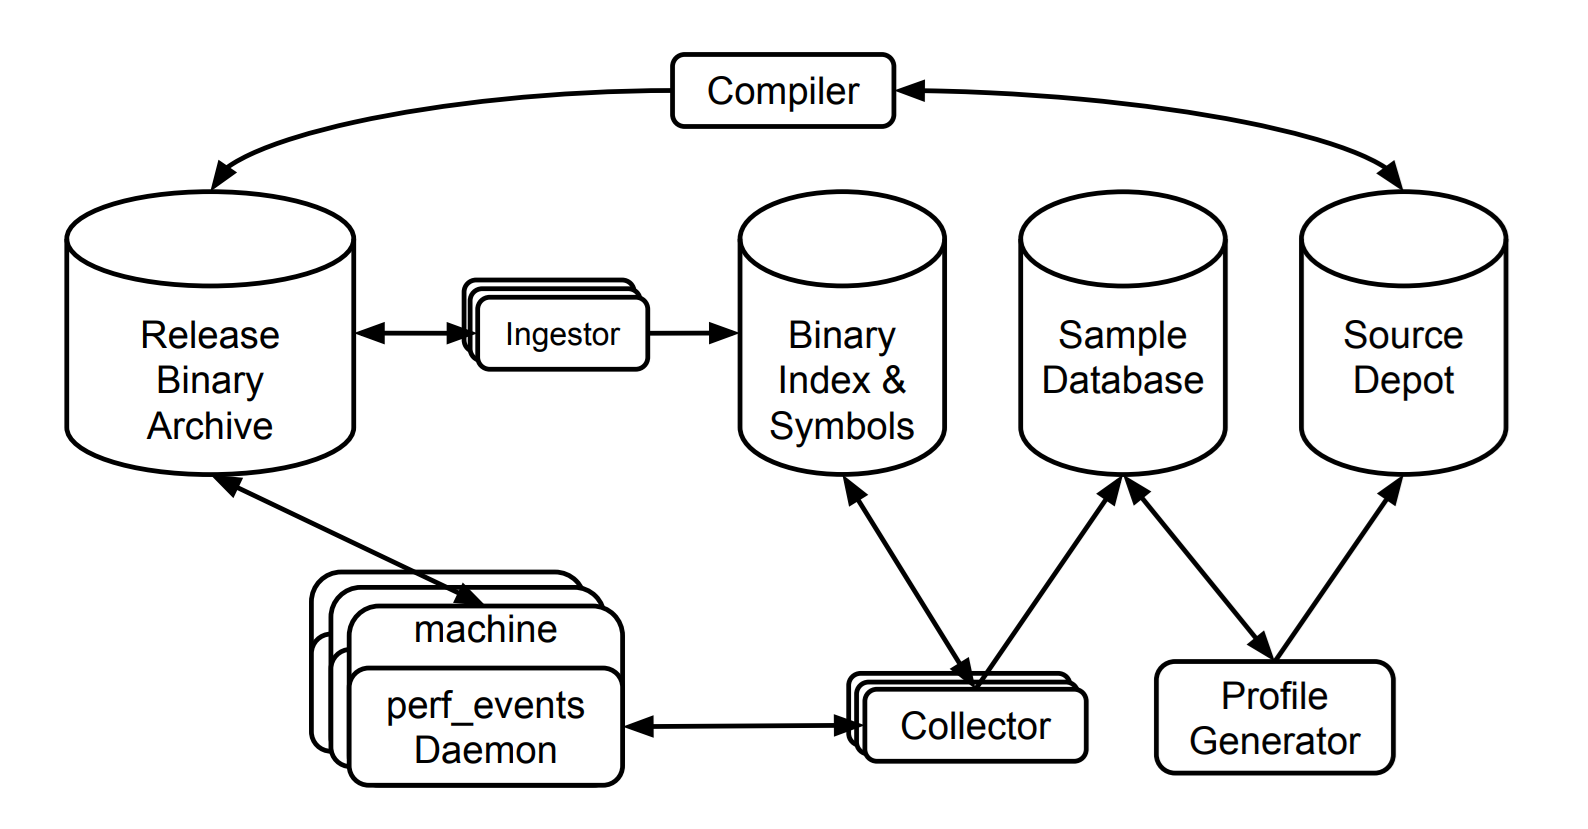
\includegraphics[scale=0.4]{PNG/FDO2}
	}
	\caption{Схема системы автоматического сбора профиля и рекомпиляции. \cite{chen2016autofdo}.}\label{partReview:fdo2}
\end{figure}

Сергей Лисицын  в своей диссертации \cite{SergeyL1} предлагает разрешить проблему зависимости профиля от входных данных с помощью версионирования отдельных участков программы, выбор между которыми делается динамически во время исполнения. Из минусов подобного решения можно отметить увеличение размеров исполняемого файла.

С популяризацией машинного обучения появилась возможность генерации качественного синтетического профиля \cite{rotem2021profile}. Авторы статьи натренировали бустинг над деревьями для генерации профильной информации, что в свою очередь позволило компилятору использовать этот профиль и применять соответствующие оптимизации. С помощью данного подхода авторам удалось добиться ускорения в 1.6 процента в среднем с максимальным результатом в 16 \%  на интерпретаторе языка Python. 
 \begin{figure}[htbp]
	\centering
	\includesvg[width = 400pt, inkscapelatex=false ]{SVG/pgowithoutprofile.drawio.svg}
	\caption{Схема компиляции с искусственным профилем.}
	\label{partReview:pgo_without profile}
\end{figure}
На рисунке \ref{partReview:pgo_without profile}а изображена тренировка модели, которая заблаговременно проводится разработчиками компилятора, а на рисунке \ref{partReview:pgo_without profile}б изображен рабочий режим, в котором работает компилятор, оказавшись у пользователя.

\FloatBarrier
